\chapter{Requirements gathering} \label{chap:ReqEng}
\textbf{Irgendwo noch artifact mit system gleichsetzen!}

This chapter determines which requirements are needed in order to solve the problem. For this purpose, the problem needs to be atomized in greater detail than its statement in the introduction. Following the relevance cycle as presented in \ref{topic:relevance cycle}, the process of gathering the requirements for the solution gives additional insights into the problem space, which in turn helps define the solution and the requirements the artifact must meet to solve the problem. The chapter discusses the methods (expert interviews and qualitative content analysis after Mayring) used to elicit the requirements and places this process in the context of the requirements development process. In the ensuing section, the data is collected in form of expert interviews and the content is qualitatively analyzed. In the third section, existing approaches to solve this problem are investigated. These approaches may serve as input for the ensuing design process. This chapter lays the groundwork for the solution definition. It serves as input for the following chapter. 

\section{Research method and objective}
The requirement gathering process for this research follows closely the requirements elicitation activity, which is an activity of requirements engineering in software engineering. Requirements engineering is a set of activities to develop and document the specifications a system is expected to meet.\footcite[Cf.][p.16]{SommervilleIntegratedrequirementsengineering2005} The information is gathered from a number of people that develop, interact with or have an interest in the system.\footcite[Cf.][p.38]{PatakiSystemRequirementsAnalysis2003} and ultimately describes what these stakeholders really need.\footcite[Cf.][p.1]{GoguenTechniquesrequirementelicitation1993}

Firstly, it is important to clearly understand what requirements are: Requirements are descriptors of what a system should do. They define the services the ideal system must provide and the constraints under which the system must operate, effectively describing the business needs to which the system responds.\footcites[Cf.][p.100]{SommervilleSoftwareengineering2011}[cf.][p.95]{IEEEIEEEstandardglossary1990} Requirements can range from high-level abstract statements of services or system constraints to very detailed functional specifications\footcite[Cf.][p.215]{DavisSoftwarerequirementsobjects1993} and often are grouped in two categories: 
\begin{itemize}
    \item \textbf{Functional requirements} A functional requirement defines a function the system must perform.\footcite[Cf.][p.34]{IEEEIEEEstandardglossary1990} It specifies how the system should react to particular inputs and how the system should behave in specific situations.\footcite[Cf.][p.102]{SommervilleSoftwareengineering2011} It defines what actions the system must do (functionality) rather than how it performs these actions. 
    \item \textbf{Non-functional requirements} A non-functional requirement refers to additional requirements which put constraints on the functionality.\footcite[Cf.][p.102]{SommervilleSoftwareengineering2011} These constraints may be a consequence of product requirements, organizational policies or external factors (e.g. reliability, standard processes, interoperability) and often apply to the whole system rather than individual features.\footcite[Cf.][p.102]{SommervilleSoftwareengineering2011}
\end{itemize}

The fact that the requirements gathering is separated from the design process helps find an objective solution. This means, that the solution is not influenced by design considerations and the requirements don't limit the implementation of the system.\footcite[Cf.][p.18]{SommervilleIntegratedrequirementsengineering2005}

These requirements are collected during the requirements elicitation phase, which is the first of a set of activities in requirements engineering.\footcites[Cf.][p.116]{SommervilleSoftwareengineering2011}[cf.][p.17]{SommervilleIntegratedrequirementsengineering2005} The requirements engineering process is somewhat ill-defined, with different authors presenting different activities and practitioners using a large number of different methods to develop the requirements.\footcite[Cf.][p.225]{ZhangEffectiverequirementsdevelopmentA2007} The main aspects of the requirements engineering process is visualized in figure \ref{fig:REAll}. The process starts with the elicitation of the requirements from a variety of knowledge sources in order to collect needed information. The requirements are consequently analyzed in order to detect overlaps and conflicts and the generated knowledge is then added to the understood knowledge.\footcite[Cf.][p.17]{SommervilleIntegratedrequirementsengineering2005} That understood knowledge serves as input for the next step, the specification, where the requirements are structured and recorded in a document (the structured requirements specification (SRS)). The documentation may be done via natural language or dedicated conceptual models, so that the requirements are clear, understandable and correct, and constitutes the final output of the overall requirements engineering process.\footcites[Cf.][p.17]{SommervilleIntegratedrequirementsengineering2005}[chapter 1]{PohlRequirementsengineeringfundamentals2011} The fourth activity comprises the validation of these requirements. It checks again if the requirements are correct and that they indeed correspond to the stakeholders' needs.\footcite[Cf.][p.17]{SommervilleIntegratedrequirementsengineering2005}
It is an iterative cycle, as inconsistent, ambiguous or missing information that is uncovered during the specification or validation steps is tried to be resolved in another elicitation session. 
Major players in the literature agree on these four main activities,\footcites[Cf.][p.225]{ZhangEffectiverequirementsdevelopmentA2007}[cf.][p.220]{DavisSoftwarerequirementsobjects1993}[cf.][chapter 1]{PohlRequirementsengineeringfundamentals2011}[cf.][p.116]{SommervilleSoftwareengineering2011} but Sommerville and Pohl and Rupp also add negotiation (reconciling conflicting stakeholders' views) and management (actively controlling the changes to the requirements) to create a full picture of the requirements engineering process.\footcites[Cf.][p.17]{SommervilleSoftwareengineering2011}[cf.][chapter 1]{PohlRequirementsengineeringfundamentals2011}


\begin{figure}
    \centering
    \includesvg[width=\textwidth]{graphics/Zhang_textcurves}
    \caption[Summary of the requirements engineering process.]{Summary of the requirements engineering process.\footnotemark}
    \label{fig:REAll}
\end{figure}
\footnotetext{With changes taken from \cite{ZhangEffectiverequirementsdevelopmentA2007}, p.225}
Since this research bases the requirements gathering on the requirements elicitation activity. The activity and the methods used to execute this activity are examined in further detail in the following paragraph. 

\paragraph{Requirements Elicitation} Requirements elicitation refers to the gathering of information to extract the requirements that the system has to fulfill. During the first activity in the requirements engineering process, possible sources of information that allow the discovery of requirements need to be identified.\footcites[Cf.][p.2]{TiwariMethodologySelectionRequirement2017}[cf.][p.17]{SommervilleIntegratedrequirementsengineering2005} These knowledge sources may be the stakeholders (users, project sponsors, managers) as presented in figure \ref{fig:REAll}, or other resources (e.g. existing systems). It is important to not only discover but to fully understand the needs of these potential stakeholders in order to communicate them to the system developers.\footcite[Cf.][p.21]{ZowghiRequirementselicitationsurvey2005} Therefore, the elicitation of the requirements is an important and critical step in the RE process.\footcites[Cf.][p.232]{ZhangEffectiverequirementsdevelopmentA2007}[cf.][p.19]{ZowghiRequirementselicitationsurvey2005} Consequently, the use of appropriate methods is imperative to a well-executed and comprehensive requirement elicitation.\footcite[Cf.][p.232]{ZhangEffectiverequirementsdevelopmentA2007}

The gathering of information, and subsequently of the requirements may be done in a multitude of ways.\footcite[Cf.][p.170]{HickeyElicitationtechniqueselection2003} Independently of which method is applied, due to the communicative nature of eliciting information, the effective communication between the researcher and the stakeholders is of key importance.\footcite[Cf.][p.1]{AlvarezDiscourseanalysisrequirements2002} These methods do not necessarily originate from a computer sciences background, instead they are mostly derived from natural sciences, knowledge engineering and practical experience.\footcite[Cf.][p.19]{ZowghiRequirementselicitationsurvey2005}

The list of available methods below is divided into categories, which roughly describe the common nature of the methods within that category: 
\begin{itemize}
    \item \textbf{Conversational methods}: Interview, questionnaire, survey\footcites[Cf.][chapter 3]{PohlRequirementsengineeringfundamentals2011}[cf.][p.170]{HickeyElicitationtechniqueselection2003}
    \item \textbf{Observational methods}: Social analysis, observation, ethnographic study\footcites[Cf.][p.227]{ZhangEffectiverequirementsdevelopmentA2007}[cf.][p.173]{HickeyElicitationtechniqueselection2003}
    \item \textbf{Creative methods}: Brainstorming, analogy techniques\footcite[Cf.][chapter 3]{PohlRequirementsengineeringfundamentals2011}
    \item \textbf{Analytic methods}: Requirement reuse, documentation study, protocol analysis, discourse analysis \footcites[Cf.][p.12]{GoguenTechniquesrequirementelicitation1993}[cf.][pp.227-228]{ZhangEffectiverequirementsdevelopmentA2007}[cf.][p.2]{TiwariMethodologySelectionRequirement2017}
    \item \textbf{Synthetic methods}: Scenarios, prototyping, joint application development, perspective based reading\footcites[Cf.][p.228]{ZhangEffectiverequirementsdevelopmentA2007}[cf.][chapter 3]{PohlRequirementsengineeringfundamentals2011}[cf.][p.3]{TiwariMethodologySelectionRequirement2017}
\end{itemize}

Conversational methods, especially interviews, form the primary method to effectively collect knowledge, because they provide means of verbal communication between the researcher and one or more stakeholders and provide for them a natural way to express their ideas, problems, and questions. On the basis of the resulting conversation, the requirements are formulated.\footcite[Cf.][pp.226/227]{ZhangEffectiverequirementsdevelopmentA2007} The observational methods put the researcher in a more passive role, where she/he observes the stakeholders in a certain situation and notes the work process, potential mistakes, risks, and open questions, which constitute the inputs for the formulation of the requirements.\footcite[Cf.][chapter 3]{PohlRequirementsengineeringfundamentals2011} Creative methods, as the name suggest, serve the purpose to discover new and innovative requirements.\footcite[Cf.][chapter 3]{PohlRequirementsengineeringfundamentals2011} Analytic methods focus on extracting requirements from existing documents, making them especially useful to quickly formulate fine-grained requirements from existing documentation.\footcite[Cf.][p.228]{ZhangEffectiverequirementsdevelopmentA2007} Finally, synthetic methods are a combination of conversational, observational, creative, and analytic techniques.\footcite[Cf.][p.228]{ZhangEffectiverequirementsdevelopmentA2007} All techniques and methods have their strengths and weaknesses, the choice therefore depends on a number of factors, for example the nature of the project, its size, or its application domain.\footcite[Cf.][p.42]{ZowghiRequirementselicitationsurvey2005}
In practice, to make use of their relative strengths and to limit their weaknesses, a combination of methods is used. 


As \cite{WhiteProbingunderstanding1992} stated: \enquote{[An] interview is the most direct method, among all the probes, of assessing a person’s understanding} His view is shared with a great number of authors in the field.\footcites[Cf.][p.174]{MacaulayRequirementscapturecooperative1993}[cf.][p.105]{SommervilleSoftwareengineering2011}[cf.][p.25]{ZowghiRequirementselicitationsurvey2005}[cf.][p.172]{HickeyElicitationtechniqueselection2003}[cf.][p.227]{ZhangEffectiverequirementsdevelopmentA2007}[cf.][p.92]{MasonQualitativeresearching2002}
Interviews were and remain the most commonly used approach to elicit information. An interview is defined as motivating the interviewee to share their information, opinion, attitude and knowledge regarding certain topics.\footcite[Cf.][p.133]{KrugerqualitativeInhaltsanalyseMethode2004} Interviews did not get this status as No.1 without reason, they allow to identify the facts and subjective opinions of the stakeholders by face to face conversation, but also to uncover conflicts or politics.\footcite[Cf.][p.2]{TiwariMethodologySelectionRequirement2017} The requirements can directly be extracted from the stakeholders' verbalized thoughts and if needed, the conversation allows further queries to treat specific topics more thoroughly and discover hidden requirements. Due to these characteristics, interviews are deemed the best approach to gather the requirements for the dashboard.

Because interviews are so popular and widely used, a number of variations have developed that may be categorized by different aspects. An interview may be closed/structured (pre-defined set of questions, looking for clear answers) semi-structured (a more flexible set of questions allowing the researcher to adapt/innovate)\footcites[Cf.][p.39]{EdwardsWhatqualitativeinterviewing2013} or open-ended/unstructured (a discussion to discover requirements together, stakeholder talks from their own perspective).\footcites[Cf.][p.2]{TiwariMethodologySelectionRequirement2017}[cf.][p.40]{EdwardsWhatqualitativeinterviewing2013} The two latter types are qualitative interviews, characterized by less structured information and more flexibility in conversation flow.\footcite[Cf.][p.13]{EdwardsWhatqualitativeinterviewing2013} These types of interviews are chosen for when the data is most feasibly generated by asking the stakeholders for their opinion and stands about certain topics.\footcite[Cf.][p.76]{MasonQualitativeresearching2002} One instant of qualitative interviews are expert interviews, which are described in more detail in the following paragraph.

% \begin{itemize}
%     \item the requirements will be extracted from expert interviews
%     \begin{itemize}
%         \item Why an interview? X
%         \item What kind of interview? explorative expert interview
%         \item What experts? Frank Bloch, Bernd Kammholz, Torsten Milsmann, Daniel Kaltenbach, Thomas Maier -> all experts in their respective field
%         \item What questions should I ask them? What do you not understand about blockchain? What would you wish to understand the most? Where do you feel lies the difficulty to blockchain and its transactions? What do you imagine under such a term as a dashboard visualizing blockchain transactions? What would be the best way to learn about it? Do you want it to be portable?
%     \end{itemize}
%     \item the interviews will be analyzed using the Qualitative Content Analysis of Mayring
%     \begin{itemize}
%         \item Why this method and not a quantitative method or different qualitative? -> Steigleider citation about how it is both the broadest and most exact technique. 
%         \item How does the analysis work? Which process steps are there?
%         \item Choose a summarizing content analysis and explain the steps for this
%     \end{itemize}
% \end{itemize}

\subsection{Expert interviews} \label{subsec:ExpertInterviews}
An expert interview is a semi-structured interview used for explorative purposes.\footcites[Cf.][p.179]{Flickintroductionqualitativeresearch2009}[cf.][p.465]{MeuserExperteninterviewkonzeptionelleGrundlagen2009}[cf.][p.31]{BognerInterviewsmitExperten2014} These purposes include 1) the orientation in a new field of research, 2) the collection of context information to complement other research methods, and 3) the development of a theory or typology by synthesizing knowledge from various experts.\footcite[Cf.][p.180]{Flickintroductionqualitativeresearch2009} The knowledge generated from these interviews is focused on a particular body of knowledge, the specific knowledge the expert has gained by specializing in a certain field.\footcites[Cf.][p.423]{BuberQualitativeMarktforschungKonzepte2007}[cf.][p.450]{PfadenhauerExperteninterviewGesprachauf2007} It gathers the expert's knowledge on their field of expertise and explicitly documents it.\footcites[Cf.][p.466]{MeuserExperteninterviewkonzeptionelleGrundlagen2009}[cf.][p.451]{PfadenhauerExperteninterviewGesprachauf2007}[cf.][p.172]{HickeyElicitationtechniqueselection2003} and even though it is a complex and elaborate method to generate data, it is applied in various fields of research due to the high quality of insights gained from the expert's knowledge.\footcites[Cf.][p.459]{PfadenhauerExperteninterviewGesprachauf2007}[cf.][p.442]{MeuserExpertInneninterviewsvielfacherprobt1991}[cf.][p.424]{BuberQualitativeMarktforschungKonzepte2007} 
%The expert interview in itself may be categorized into four different types depending on the interview's purpose.

The type of expert interview led during this research is of explorative nature. It helps gain insights into the problem space, and thus allows the better definition of the problem and the generation of hypotheses on how to solve this problem.\footcite[Cf.][p.28]{BognerInterviewsmitExperten2014} The main goals of this type of interviews are 1) to collect relevant information about the research environment and the problem space as well as 2) to discover the experts' opinion and attitudes regarding that problem.\footcite[Cf.][pp.28/29]{BognerInterviewsmitExperten2014} Therefore, this type of interview is well suited for the purpose of gathering the requirements for the artifact as well as to collect more information regarding the problem. Other variants of expert interviews are of systematizing (systematic extraction of knowledge regarding a particular topic), sustaining (scientific definition, explanation and connection of terms on the basis of the expert's knowledge) or theory-generative (discovery of implicit decision criteria, routines, or world views on the basis of the expert's subjective opinion) nature.\footcites[Cf.][pp.27-30]{BognerInterviewsmitExperten2014}[cf.][p.421]{AghamanoukjanQualitativeInterviews2007}[cf.][p.180]{Flickintroductionqualitativeresearch2009}

But who exactly may call themselves an expert? The answer to the question, what defines an expert varies on the issue and the approach taken in the study of this issue.\footcite[Cf.][p.179]{Flickintroductionqualitativeresearch2009} As stated by \cite{MeuserExpertInneninterviewsvielfacherprobt1991} (p.444), being an expert is a relational status depending on the interest/purpose of the study. An expert may be any person, who has distinguished knowledge in a particular subject and thus acts as a body of authority on that particular field. This knowledge, whether it stems from practical experience or in-depth study, allows the clear identification of a problem space and the formulation of meaningful instructions for others to solve that problem.\footcites[Cf.][p.469]{MeuserExpertInneninterviewsvielfacherprobt1991}[cf.][p.467]{MeuserExperteninterviewkonzeptionelleGrundlagen2009}[cf.][p.179]{Flickintroductionqualitativeresearch2009}[cf.][p.451]{PfadenhauerExperteninterviewGesprachauf2007}[cf.][p.19]{BognerInterviewsmitExperten2014} The quality to detect not only a problem and its causes, but also its potential solutions is what distinguishes an expert from a specialist.\footcite[Cf.][p.424]{BuberQualitativeMarktforschungKonzepte2007}  

As suggested by Meuser and Nagel, a compendium of questions is used as the basis for the interview.\footcite[Cf.][p.472]{MeuserExperteninterviewkonzeptionelleGrundlagen2009} The compendium's purpose is to provide an orientation for the researcher to not loose track of what information is needed. During the interview, the interviewee is motivated to speak freely, therefore the researcher should not ask too standardized questions but rather try to have a flexible conversation with the expert about the field of interest. However, they must not forget what information they are actually looking for. The compendium serves in that sense as a guideline; it reminds the researcher of the interview's purpose. The compendium of questions supports the main objective of the interview, to extract and understand the expert's opinion, but it is not an end in itself. The researcher must adapt the pre-formulated questions accordingly to react to the conversation flow. Additionally, the preparation of the compendium allows the researcher to prepare and structure the interview beforehand and to gain enough competency about the interviewee's field of expertise to enable a productive conversation.\footcites[Cf.][p.472 et seqq]{MeuserExperteninterviewkonzeptionelleGrundlagen2009}[cf.][p.133]{KrugerMethodennaturwissenschaftsdidaktischenForschung2014}[cf.][p.431 et seq]{BognerInterviewsmitExperten2014}[cf.][p.123 et seqq]{NiebertLeitfadengestutzteInterviews2014}[cf.][p.421]{AghamanoukjanQualitativeInterviews2007}
To ensure the compendium can effectively applied, it should meet the following requirements: 
\begin{itemize}
    \item \textbf{Clear}: The compendium has a clear and open layout. The questions guide the interviewer, they should not distract from the conversation.
    \item \textbf{Not overloaded}: The number of questions stays limited to allow a conversation. Too many simple questions render the expert 
    \item \textbf{Logically structured}: The compendium is logically structured, so that the interviewer knows to which topic he should lead the conversation. Note that the interviewee's narrative and thoughts may not follow this structure and it is up to the interviewer to adapt accordingly.
    \item \textbf{Appropriate language}: The questions are formulated in a language that is common to both interviewer and interviewee. Use of technical jargon may complicate or obstruct the conversation/information gathering.
    \item \textbf{Guiding}: The questions collected in the compendium guide and not restrict the conversation. It is of course acceptable for the conversation to go a different way than the interviewer has expected.\footcite[Cf.][p.126]{NiebertLeitfadengestutzteInterviews2014}
\end{itemize}

The process of interviewing an expert is presented in the following list and summarized in figure \ref{fig:InterviewProcess}:
\begin{enumerate}
    \item \textbf{Finding questions}: The process starts with the collection of all research questions and hypotheses regarding the study. The main research questions the study aims to resolve are atomized in smaller questions.
    \item \textbf{Grouping questions}: Selected questions are sorted and grouped in bigger blocks with each block pertaining to a particular aspect of study.
    \item \textbf{Defining questions for the compendium}: Following the requirements outlined above, a subset of questions is put in the compendium.
    \item \textbf{Cross referencing and refinement}: The effectiveness/utility of the developed catalogue of questions is tested by conducting a test interview beforehand and ensuring that the asked questions reflect the initial research questions. The compendium is hence refined iteratively until it is deemed appropriate for actual use.
    \item \textbf{Sampling}: The experts to be interviewed are chosen. The selection of these experts depends on a number of factors, ranging from the subject of study, the quality of data, the study design to the availability of possible respondents.\footcites[Cf.][p.134]{KrugerqualitativeInhaltsanalyseMethode2004}[cf.][p.1 et seq.]{MorseDeterminingsamplesize2000}[cf.][p.137]{Flickintroductionqualitativeresearch2009}
    \item \textbf{Conducting the interviews}: The interview is done in an open manner to entice an interesting and meaningful conversation.
    \item \textbf{Content analysis}: The interviews are transcribed and analyzed. The analysis may focus on quantitative and/or qualitative information in order to extract useful information from the conversation.\footcites[Cf.][p.37 et seqq]{BognerInterviewsmitExperten2014}[cf.][p.454 et seqq]{MeuserExperteninterviewkonzeptionelleGrundlagen2009}[cf.][p.72]{MasonQualitativeresearching2002} Depending on the method of content analysis chosen, this step is divided into further activities.\footnote{For more information, see \ref{subsec:Mayring}}
\end{enumerate}

\begin{figure}
    \centering
    \includesvg[width=\textwidth]{graphics/InterviewProcess}
    \caption[The interview process]{The interview process}
    \label{fig:InterviewProcess}
\end{figure}

The methodological analysis of the conducted interviews is essential to extracting the needed information from the conversation, however, the process does not define an exact instruction on how to perform this analysis. For this purpose, the method of qualitative content analysis after Mayring is chosen/consulted, which is described in the following subsection.

\subsection{Qualitative Content Analysis} \label{subsec:Mayring}
A methodological approach to evaluate the conducted interviews is key to ensure the correctness and completeness of the information. Since the purpose of the interviews is to collect qualitative data and not to compare the key messages from each expert with one another, a qualitative method is appropriate in order to generate a general statement regarding the requirements of a possible solution.\footcite[Cf.][p.456]{MeuserExpertInneninterviewsvielfacherprobt1991} There exist a number of different text analytical approaches, from which the qualitative content analysis after Mayring seems to be the broadest (describing a wide set of different procedures) and most exact one (prescribing clear step- by-step models and analytical rules). \footcite[Cf.][p.197]{SteiglederstrukturierendequalitativeInhaltsanalyse2008} Its purpose is to systematically generalize the statements from the conversation in order to allow a conclusion to be drawn.\footcite[Cf.][p.13]{MayringQualitativeContentAnalysis2014}
In general, qualitative data analysis can be structured into three activities that themselves have different steps: the 1) gathering, 2) processing, and 3) evaluation of the material.\footcite[Cf.][p.135 et seqq]{KrugerqualitativeInhaltsanalyseMethode2004} Processing the material includes the transcription and redaction of the conversation. Transcription of the conversation may be done in different ways, depending on which information are of interest to the researcher. There exist methods which handle dialect, verbal and non-verbal expressions through special signs, exclude unnecessary sections of the interviews (selective transcription), or transcribe the whole conversation as it occurred (verbatim transcription).\footcite[Cf.][p.44 et seq]{MayringQualitativeContentAnalysis2014} As the analysis is based on the transcripts, clear transcription rules need to be employed consistently in order to accurately represent the raw material.\footcite[Cf.][p.44]{MayringQualitativeContentAnalysis2014} The third activity, evaluation, may be further divided into the sorting/arrangement of statements, the explication and the structuring of single statements. The qualitative content analysis expands on these activities in so far as that it defines an eleven-step process allowing its application as a scientific method because this process is testable, transferable to other subjects and available for use by others.\footcite[Cf.][p.53]{MayringQualitativeContentAnalysis2014}
 
The analysis utilizes qualitative and quantitative steps and may therefore be categorized as a mixed methods approach.\footcite[Cf.][p.10]{MayringQualitativeContentAnalysis2014}

Mayring defines the process, presented in figure \ref{fig:MayringProcess}, as follows: 
\begin{enumerate}
    \item \textbf{Definition of the material}: The material on which the analysis is based must be defined exactly. The defined set of material is not to be changed during the analysis.
    \item \textbf{Analysis of the situation of origin}: The circumstances and the setting in which the material is collected needs to be described. This description includes the participating parties, the socio-cultural background, the place where the collection takes place, as well as how the material is collected.
    \item \textbf{Formal characteristics of the material}: This step documents the form of the material that is analyzed. A possible description may be: \textit{selective transcripts}
    \item \textbf{Direction of analysis}: The focus of the interpretation is defined. By stating which type of information is of interest and why, it is made clear why other aspects are left out of the analysis.
    \item \textbf{Theoretical differentiation of sub-components of the problem}: This step is characteristic for the qualitative content analysis. It documents the research questions that characterize the analysis and states their importance based on the respective literature.
    \item \textbf{Determination of techniques of analysis and establishment of a concrete procedural model}: Mayring has identified a set of different analysis techniques that may are either a form of summary (create a comprehensive overview), explication (increase understanding of particular text passages), or structuring (assess the material regarding pre-defined criteria). The technique chosen further defines the steps thereafter.
    \item \textbf{Definition of content analytical units}: There are three types of content analytical units that are used for segmentation in a latter step: the coding unit (smallest component of material which defines the sensitivity of the analysis), the context unit (the largest text component that may fall within one category), and the recording unit (decides which text components are to be analyzed and the order of the analysis).
    \item \textbf{Analytical steps taken by means of the category system}: These steps depend on the analysis technique chosen and are described in a following paragraph. Common to all techniques is the creation of a category system that is used to analyze the material.
    \item \textbf{Re-checking the category system}: The category system is applied to the material and other bodies of literature on the study with the intention to reduce the number of categories and refine the category system. 
    \item \textbf{Interpretation of the results}: The results of the analysis are interpreted with respect to the underlying research question in order to gain a comprehensive, generalized answer to that question.
    \item \textbf{Application of content-analytical quality criteria}: As with any scientific method, quality controls must be applied in order to assess the objectivity, reliability and validity. Therefore, the analysis is judged by its semantical validity, sampling validity, predictive validity, construct validity, stability, reproducibility and accuracy.\footcites[Cf.][p.40 et seqq]{MayringQualitativeContentAnalysis2014}[cf.][p.280]{Flickintroductionqualitativeresearch2009}
\end{enumerate}

\begin{figure}
    \centering
    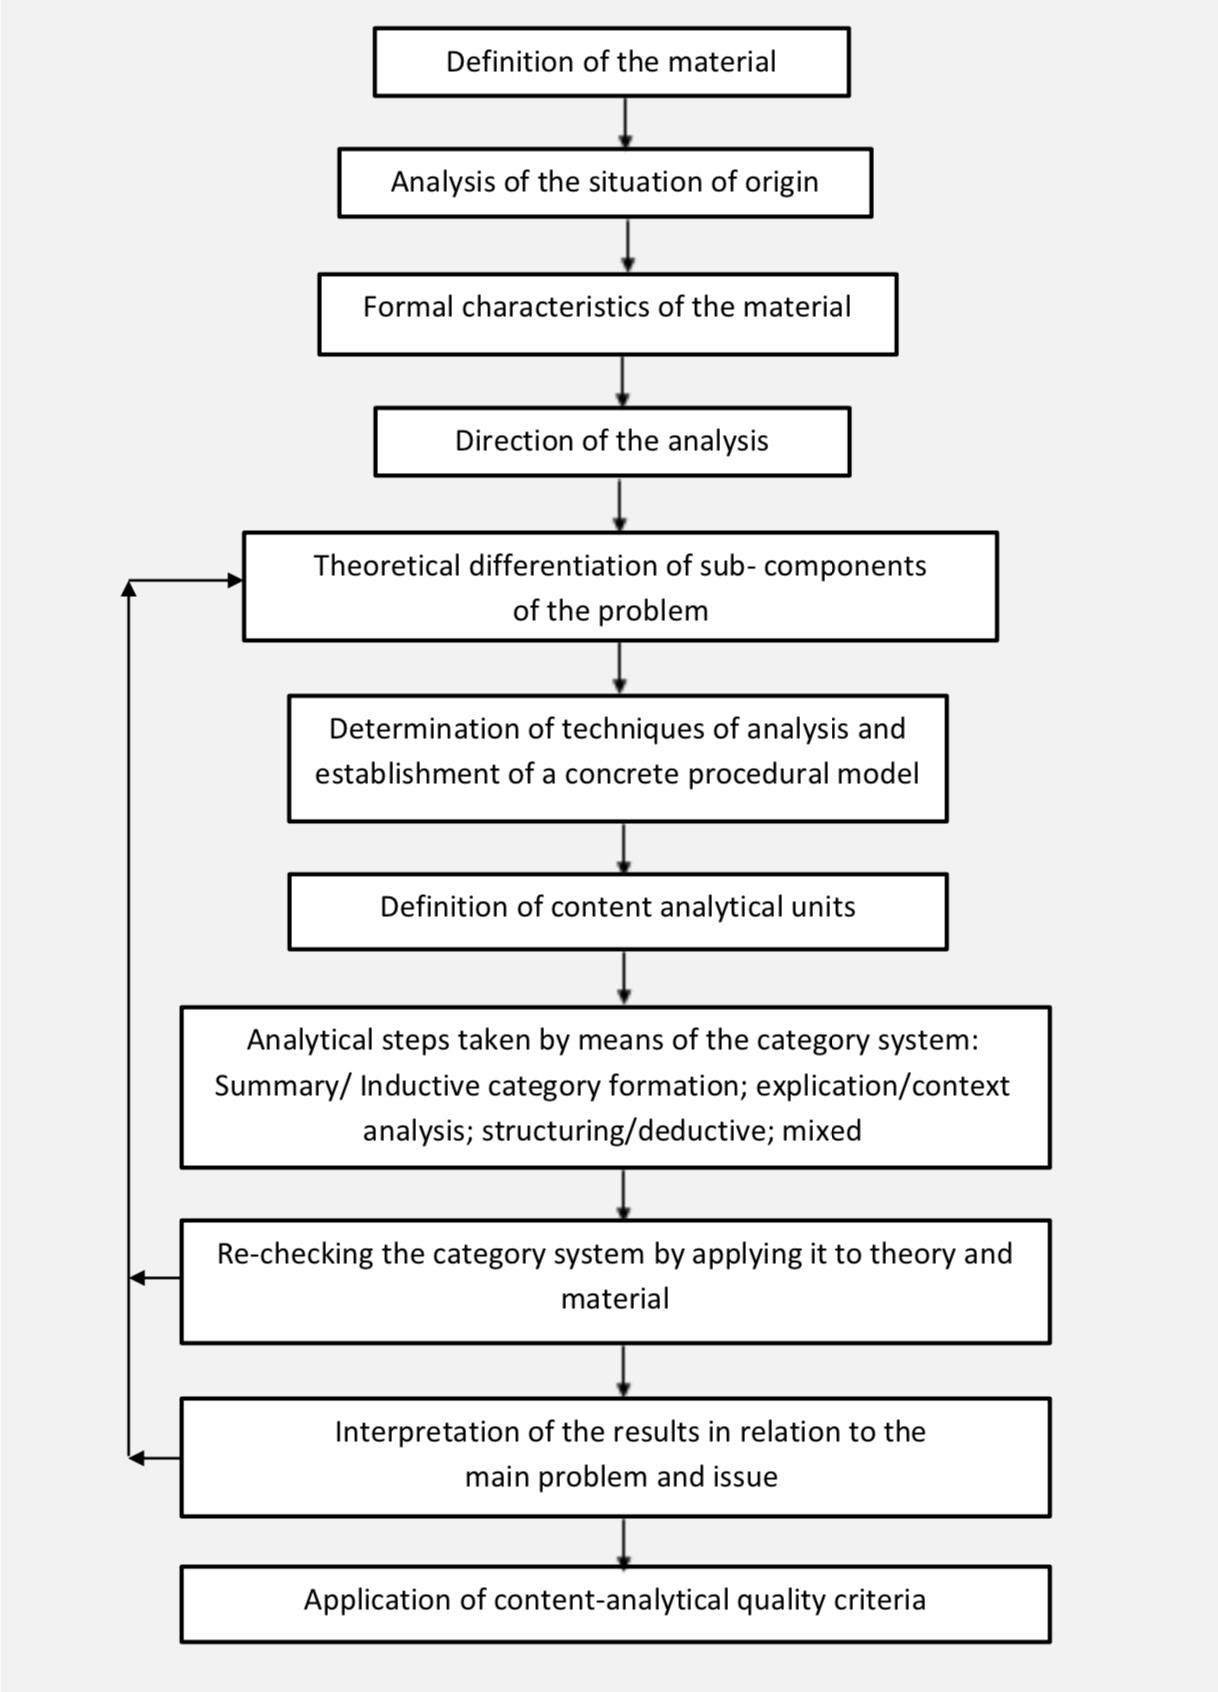
\includegraphics[width=0.8\textwidth]{graphics/MayringProcess.png}
    \caption[The general model of the content-analytical process.]{The general model of the content-analytical process.\footnotemark}
    \label{fig:MayringProcess}
\end{figure}
\footnotetext{Taken from \cite{MayringQualitativeContentAnalysis2014}, p.54}

This process serves as a model and must be adapted to fit the material and the specific research problem. For this study, the purpose of the analysis is to extract information regarding the problems and struggles, the interviewees experience when trying to understand the blockchain technology. For this purpose, the material is summarized, which creates an abstraction from the material that correctly represents/generalized said material. \footcite[Cf.][p.68]{MayringQualitativeContentAnalysis2014} The summarizing technique is comprised of four steps: 1) Paraphrasing the content-bearing text components, 2) generalizing these to a certain abstraction level, 3) reducing these in a first attempt to remove semantically identical paraphrases and 4) reducing these a second time through binding and integration of paraphrases on the envisaged abstraction level. After these steps are completed, the new statements are put into the category system (step 8), whose exactness/applicability is tested after 10-50\% of material has been sighted. If the level of abstraction does not meet the desired level, the category system must be revised and all information re-evaluated.\footcite[Cf.][p.68 et seq]{MayringQualitativeContentAnalysis2014}

This analysis of the interviews corresponds to the evaluation activity of the requirements development process (see figure \ref{fig:REAll}) and provides the basis to subsequently specify the requirements for the desired artifact. 

\section{Data collection via Expert Interviews}
This section applies the defined methods of requirements elicitation (interviewing and content analysis) to the research problem in order to define the problem in a more detailed fashion and extract the requirements needed to solve this problem. 
The explorative expert interview is ideally suited for the purpose of requirements gathering regarding the dashboard design process, because collecting a rather broad palette of information to explore why the problems in understanding blockchain transactions exist and how they might be solved, provides a solid basis from which requirements may be derived in a reliable manner. By leading an open, little standardized conversation, that looks to a question compendium for guidance, the expert's are free to state their opinion regarding the problem.
\paragraph{Design of the question compendium} Following the interviewing process as presented in \ref{subsec:ExpertInterviews} and figure \ref{fig:InterviewProcess}, the study's research question \textbf{What should the artifact visualize so it explains the blockchain technology in a comprehensible way?} serves as foundation from which the catalogue of questions is derived. Naturally, the researcher has some kind of expectations towards the interviews and their results, which might influence the design of the compendium. In order to acknowledge this bias (expectations regarding the answers to certain questions), the compendium is divided into three columns. The first column lists all major guiding questions, which serve as orientation for the interviewer during the interviews. The second column should contain the expected answers to these questions, formulated by the researcher before the interviews take place. Finally, the third column contains additional questions the interviewer might ask in case their expectations are not met.\footcite[Cf.][p.431]{AghamanoukjanQualitativeInterviews2007}

HIER DIE FRAGEN

\paragraph{Sampling} The following step comprises the selection of experts to be interviewed which is based on purposive expert sampling (the researcher relies on their judgment to choose the set of participants from a population of possible experts/the selection is based on the relevance for the theory to be developed)\footcites[Cf.][p.137 et seqq]{Flickintroductionqualitativeresearch2009}[cf.][p.16]{EdwardsWhatqualitativeinterviewing2013} However, because this method is vulnerable to errors by the judgment of the researcher and may be subject to high level of bias, the selection must be well argued for in order to be accepted as representative. \textbf{Die purposive Sampling Methode am Ende auch kritisieren!} The participants have to meet the following requirements to be accepted as "good informants"\footcite[][p.73]{MorseDeterminingsamplesize2000}: have the necessary knowledge to answer the questions, have the capability to reflect and articulate, be available and ready to participate.\footcite[Cf.][p.138]{Flickintroductionqualitativeresearch2009} Regarding the size of the set to be interviewed, sources agree to disagree.\footcites[Cf. in addition][p.1]{MorseDeterminingsamplesize2000}[cf.][p.134]{KrugerqualitativeInhaltsanalyseMethode2004} The study of Baker et al \textit{How many qualitative interviews is enough?} collected a number of renowned social scientists' and academics' opinions and found out that the general accord was that the sample size depends on different factors.\footcites[Cf.][p.4 et seqq]{BakerHowmanyqualitative2012} In general, the sample size should be as big as needed to reach saturation and representation of the population, but in the case of purposive sampling, the statistical representatibility is not of interest.\footcite[Cf.][p.144]{MasonQualitativeresearching2002} That is because the purpose of the sample is to provide a broad basis of experts who have knowledge on the possible use cases for blockchain or who are aware of what other persons are missing in understanding of the blockchain technology.

The experts chosen are middle-level managers at HPE, all working in areas that might be positively or negatively affected by developments in the blockchain area. The experts have knowledge in their respective field of work and understand that blockchain has the potential to disrupt their client's processes. They know how their clients could benefit of blockchain and therefore may know what information is important to them.

The sample size is 5 because these were the only experts meeting the requirements and available during the time frame of the requirements elicitation phase.

\paragraph{Transcription} The transcribed documents are in the appendix. The transcription used is a comprehensive approach, which means that 

In addition to the information from the expert interviews, the internet and academic literature is searched for existing approaches to visualize and explain blockchain technology. These existing approaches may give insights and ideas what to include (and at what abstraction level) in the dashboard. This research is done in the following section.

\section{Gathering existing solution approaches}